\section{\ours{}: Mixed-Initiative Collaborative Robot}
\label{sec:method}

\begin{figure*}[t!]
    \centering
    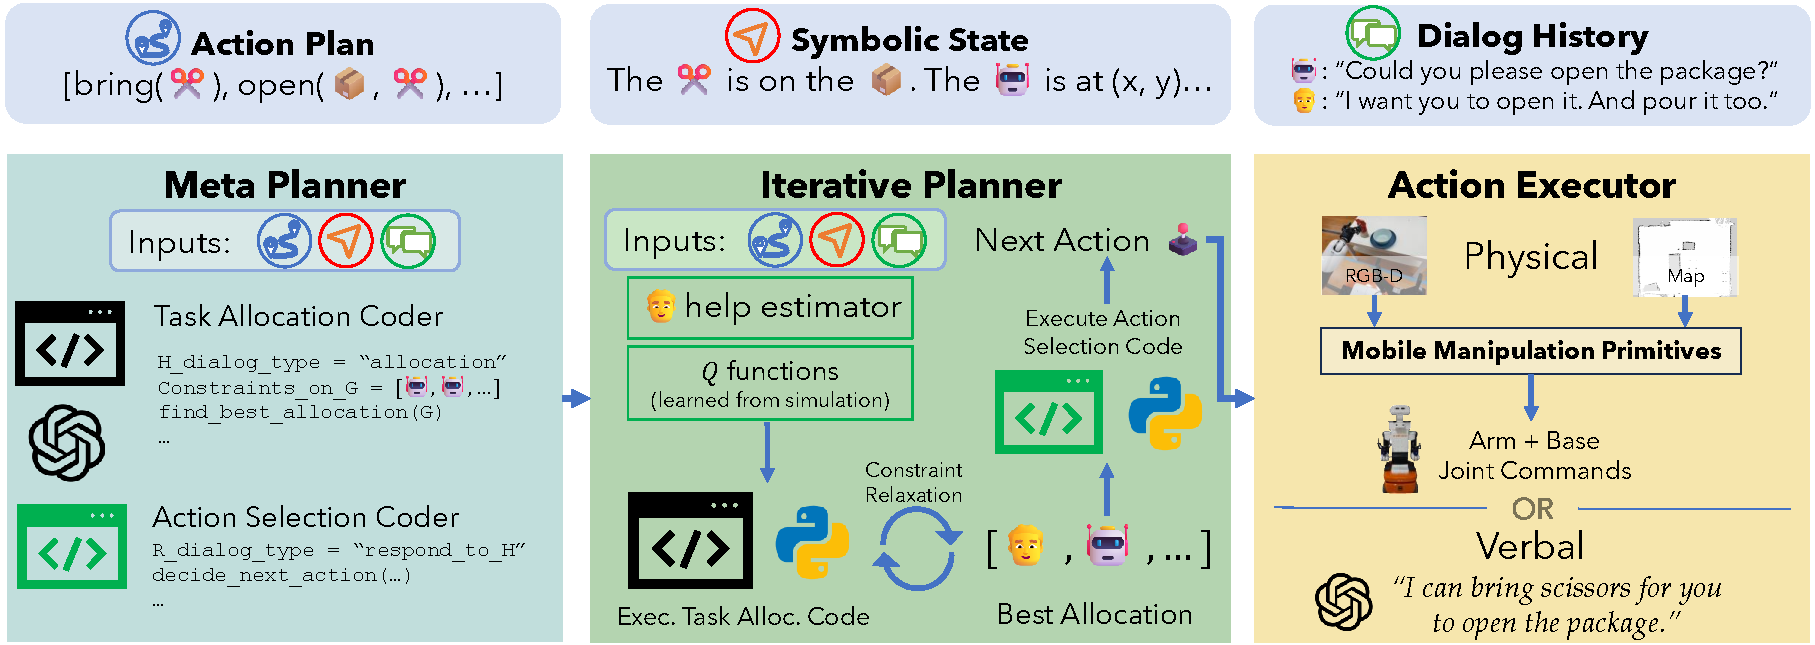
\includegraphics[width=1\textwidth,trim={0 0.0cm 0 0},clip]{figs/fig3_v4.pdf}
    \caption{\ours{} consists of 3 decision-making modules: a meta-planner that produces a collaborative strategy expressed through adaptive planning code, a planner that executes the code and optimizes our objective (Eq.~\ref{eqn:objective}) to decide the next primitive action, and an action executor that outputs the low-level pose trajectory or verbal utterance to say to the human.
    }
    \label{fig:sys-arch}
\end{figure*}


% \subsection{Optimization Formulation}
\subsection{Collaborative Task Allocation as Optimization.} 

A helpful physical collaborator must aim for task success with minimal human effort while adhering to human preferences expressed in dialog (i.e., for certain steps to be done by a certain agent). Therefore, we formulate our objective for collaborative task allocation as a constrained optimization problem, where constraints are updated based on dialog exchanges.
To avoid a complex multi-objective formulation, we combine success probability and effort into a single Q-value by
building on prior work on temporal distances in RL~\cite{myers2025learningtemporaldistancescontrastive}. Then, to allocate task steps, \ours{} compares robot and human Q-values.

We assume each task step is executed by a multi-task policy $\pi$ that performs continuous low-level control at a fixed control frequency. In this low-level MDP (distinct from the high-level task MDP described in Sec.~\ref{sec:prob-setting}), we define the reward as $r = -1$ per time step until the skill completes or times out, at which point $r_{\mathit{termination}} = 0$. A well-trained Q-function, $Q: o_t \times a_t = (\omega_t, \theta_t) \mapsto \mathbb{R}$ with a discount factor of 1, thus represents the \textbf{negative expected number of timesteps} until skill completion from a given state.
For a perfectly competent agent (i.e., human), this corresponds to the average timesteps required to perform the action.
For an imperfect agent that may fail, the Q-function reflects a weighted expectation over both successful and failed outcomes—where failure contributes a significant timestep penalty (timeout) weighted by its probability. We assign each agent a distinct Q-function: $Q_R$ for the robot and $Q_H$ for the human.
These agent-specific Q-functions thus provide a unified, interpretable cost metric for comparing step allocations, jointly capturing both execution time (effort) and likelihood of success.

% If we optimize based on the formalism above, our agent would consider human and robot effort to be equally valuable, and that if a step is assigned to a human, it will always be successfully executed.
% This is however 

However, directly optimizing step allocation using only these two Q-functions diverges from realistic human-robot collaboration scenarios in three ways:
(1) human and robot effort are valued equally, ignoring the higher worth of human time and attention;
(2) the human is assumed to always comply with robot-initiated requests, overlooking variability in willingness or availability; and
(3) human-initiated requests or preferences are not considered, limiting the system’s adaptability to human intent.
To address (1), we introduce a \textit{human-effort factor}, $\alpha$, a ratio valuing human effort to robot effort. % If the human would rather spend up to 10 seconds to perform a task that takes the robot 100 seconds, then $\alpha = 10$.
To address (2), human Q-values are adjusted with an inferred probability, $p_{H,t}$, of the human agreeing to perform action $a_{H,t} = \omega_t(\theta_t)$ when asked.
For less cooperative users, this probability lowers the expected success of $a_{H, t}$, effectively increasing the magnitude of the negative Q-value due to potential human refusal. To address (3), we enforce constraints, $C_1,\ldots,C_n$, extracted from human-initiated dialog—such as explicit requests to perform specific steps themselves or delegate them to the robot.
Altogether, we propose the following objective to find the optimal task allocation $G^*$:
\begin{equation}
\label{eqn:objective}
\begin{aligned}
\max_{g_t, ..., g_T} \quad & \sum_{t}^{T-1} \left( \mathds{1}_{g_t = H} \cdot \frac{\alpha}{p_{H, t}} + \mathds{1}_{g_t = R} \right) Q_{g_t}(s_t, a_t),\\
{s.t.} \quad & C_1, \ldots, C_n \text{ are satisfied}\\
\end{aligned}
\end{equation}
% G \in \{R, H\}^{T-t}

% \roberto{feels weird to end section on math.}That is, the algorithm searches for an allocation $G$ that will minimize execution time weighted by human effort, subject to the human's expressed constraints. 
that minimizes expected time-to-success and human effort.


\subsection{\ours{} Framework}
% Developing a complete and helpful collaborative robotic solution requires solving multiple problems:
% It first requires finding a good task allocation by solving the optimization problem above, which involves parsing previous dialog with the human to infer constraints, estimating the capabilities of each agent (Q-functions) to perform different steps, and inferring the human's willingness to help.
% Second, it requires negotiating with a human to handle the step allocation through verbal actions via robot-initiated dialog.
% Third, it also requires executing physical actions for some steps.
% And fourth, it requires incorporating any new requests from the human via human-initiated dialog and adapting to their willingness to help.
% With an optimization formulation in hand, we now discuss how our method interfaces with the main communication paradigm we have advocated for: mixed-initiative dialog. 
\methodname{} is a three-level framework (Fig.~\ref{fig:sys-arch}) that includes 1) a meta-planner that processes human dialog and generates a collaborative strategy expressed in code, 2) an iterative planner that updates planning state variables and allocates and decides the next action to perform by executing the code, and 3) an action executor that carries out the action primitive, either through low-level physical actions or by formulating a dialog utterance to the human.

\textbf{L1: Meta-planner.} The meta-planner produces adaptive planning code that dictates the overall strategy for L2 and L3 to follow. 
Based on the most recent human dialog, the current symbolic state of the world, the task plan, and approximately 15 in-context learning (ICL) examples, it generates two pieces of code: first, \textbf{task allocation} code to adapt the optimization computation, such as to map human dialog into additional constraints, and second, \textbf{action selection} code for how to choose the next action, such as whether to engage in additional dialog, proposals to split up the task with the human, or negotiation rounds before proceeding further with physical steps in the plan. The meta-planner is implemented as an LLM-based (GPT-4o) coder, and prompts can be found on our project website.\footnotemark[1]
% For instance, if the human rejects the robot's previous help request for a high-level abstract step, the meta-planner %turns on a boolean variable for the planner to 
% will try to split the abstract step into a few low-level steps and request help for a subset of these low-level steps. If the human initiates dialog, the meta-planner will convert the human's intent into constraints, expressed as a code array lined up with the remaining plan steps, for the planner to follow.

\textbf{L2: Iterative Planner.} 
The iterative planner runs code from the meta-planner (L1) to make two key decisions: whether to initiate dialog and which verbal or physical action to perform. L2 runs in two stages. \textit{First}, it performs constrained optimization to find the best task allocation for the remaining task steps. To do this, we evaluate Eq.~\ref{eqn:objective}  under all possible task allocations fulfilling the constraints. Initially, the planner attempts to incorporate all constraints from the mixed-initiative dialog history. If no feasible allocation is found (e.g., human asked the robot perform a step it is incapable of), the planner iteratively relaxes the most recent constraint, and the robot verbally explains its incapability.

To quantify Eq.~\ref{eqn:objective}, \methodname{} requires accurate Q-functions that capture each agent’s expected effort and success probability on each task step. To collect data to learn the robot's Q-function ($Q_R$), we use the OmniGibson simulator~\cite{li2022behavior}, configured with a coarse model of the real-world task, environment,
% Appendix Reference: (see \ref{app:ours-details} for visualizations).
and action primitives, recording both completion times and success rate. 
% These statistics are used to construct $Q_R$ as described earlier in this section.
We train a supervised network as $Q_R$ that predicts the expected timesteps for an action primitive $a$ to succeed from a given symbolic state $o$.
Conditioning $Q_R$ on symbolic states minimizes the sim-to-real gap when we deploy the function to our real-world setting. When estimating the human's Q-function ($Q_H$), we assume perfect competence (i.e., no execution failures).
Thus, we simply obtain time estimates for each step from an LLM predicting how long a human needs to execute action $a_t = \omega_t(\theta_t)$, plus a travel time estimate based on human-object distances.%—assuming an average walking speed of 1.4m/s.

To adapt to changing human helpfulness, \ours{} estimates the probability of human assistance at the current $t$-th timestep, $p_{H,t}$, using an LLM-based sentiment analysis over prior human-robot dialog. This enables \methodname{} to adapt to temporally-changing user sentiments. %unhelpful humans—thereby avoiding unnecessary delays due to failed help requests.
After deciding the optimal task allocation, the second stage of L2 executes meta-planner action selection code to generate the optimal action $a = \omega(\theta)$ to execute: a physical mobile manipulation primitive $\omega$ to perform a task step on objects specified in $\theta$, or a verbal primitive $\omega$ to initiate dialog to ask for help, propose splitting up steps, or respond to human-initiated dialog regarding specific task steps specified in $\theta$.
% This action may be verbal—initiating or responding to human dialog—or physical—executing a manipulation primitive to complete part of the task.

% The iterative planner executes the code from the meta-planner at two steps. \textit{In the first step}, it executes the optimization code that enumerates all possible task allocations and chooses the one that maximizes Eq.~\ref{eqn:objective}. For this computation, the planner instantiates the Q-functions based on the actions and the current state (see below on how the Q-functions are pretrained), and the probability of human help, $p_{H,t}$, based on a LLM-based sentiment analysis over prior human-robot dialog. By changing $p_{H,t}$ dynamically, \methodname{} can adapt to helpful or uncooperative humans by raising the optimization cost to assign actions to them, avoiding losing time requesting their help.
% This enables our system to adapt quickly to a wide variety of human collaborators whose predilection for helping the robot may itself fluctuate over time. An increasing $p_{H, t}$ would decrease human Q-values and may encourage the robot to allocate more tasks to the human, and a decreasing $p_{H, t}$ would do just the opposite.
%$p_H,t$ based on prior human-robot dialog. 
% In the initial iteration of the planner, the optimization code incorporates all constraints generated by the meta-planner based on the mixed-initiative dialog history. However, if no feasible allocation is found—e.g., when the human requests to assign a step to the robot that it cannot perform—the constraints derived from the most recent human verbal action are iteratively relaxed.

% Once the optimal allocation has been found, \textit{in the second step} the planner runs the meta-planner code that forms the optimal action $a$ to execute as response, 
% including the type of primitive, $\omega$, and its parameters, $\theta$.
% This can be a verbal action to initiate or reply to human initiated conversation, or a physical action to perform part of the manipulation task.



% If the planner determines that the robot should respond to the human, the next action is set to ``converse'' (e.g., informing the human about unsatisfiable requests).
% Otherwise, the planner either executes the next physical action $\omega_t(\theta_t)$ itself or verbally requests that the human perform it.

% Fault recovery
% Sometimes, the code produced by the meta-planner is not executable. For fault recovery, the meta-planner is re-queried up to 2 additional times to create code. If these attempts also produce non-executable code, the most recent dialog from the human is ignored for 2 further meta-planner requeries.

\textbf{L3: Action Executor.} The action executor performs the action primitive selected by the planner (L2). For \textit{physical actions}, it generates a trajectory for navigation and arm movement to reach the location of and manipulate the target object while avoiding obstacles. We build a pipeline similar to \cite{shah2024bumble} that uses the \texttt{move\_base} ROS package for navigation path planning over a 2D occupancy map, and Grounding DINO~\cite{liu2023grounding} to segment the target object from an open-world scene based on the object specified in $\theta$. We backproject segmented image pixels from RGB-D camera data into a 3D point cloud to identify graspable or placeable points in the robot’s workspace that the arm reaches through inverse kinematics (IK). For \textit{verbal actions}, an LLM generates free-form natural language utterances to communicate with the human based on the dialog intent $\omega$ and verbal action parameters $\theta$ decided in L2. The LLM uses 10 ICL examples to generate language grounded in the context of the task and dialog.

% Summing these two components yields a Q-value estimate for the human for each step in the task plan.
% If the human initiates dialog and volunteers to perform a future step, we set the corresponding Q-value to zero for all subsequent planning iterations, as the human cost for that step no longer needs to be considered. 


% that preserves the relative distances between task-relevant furniture and objects. We collected data in the form of $(o_t, \omega_t (\theta_t), \mathcal{T})$, where $\mathcal{T}$ is the number of low-level timesteps for the robot to successfully complete action $\omega_t(\theta_t)$ from the robot's location $o_t$. For failed rollouts, we set $\mathcal{T}$ to some large constant number, so that the average $\mathcal{T}$ of all the rollouts gives us a signal about not just how long an action primitive takes to execute, but what its success rate is from some state $o_t$. We fit a shallow Q-network to these samples via regression, and transfer these networks to our real-world system. To avoid the sim2real gap, we used a low-dimensional observation $o_t$ (symbolic state and robot position), instead of a more fine-grained image observation.


% \textbf{Human Q-functions.} We prompt the LLM to estimate the time a human would take to complete a given step $\omega_t(\theta_t)$.
% Additional, we add an estimated travel time, computed by dividing the distance from the human’s current position to the target object’s location by an average walking speed of $1.4 \text{m}/\text{s}$.
% Summing these two components yields a Q-value estimate for the human for each step in the task plan.
% If the human initiates dialog and volunteers to perform a future step, we set the corresponding Q-value to zero for all subsequent planning iterations, as the human cost for that step no longer needs to be considered.

% \textbf{Inferring the probability of human help.} To estimate the probability of the human helping on a current timestep $p_{H, t}$, we rely on the sentiment understanding of LLMs to reason about the proportion of previous requests the human accepted from the robot, and whether the human seemed eager or reluctant to help out the robot in its previous requests. This enables our system to adapt quickly to a wide variety of human collaborators whose predilection for helping the robot may itself fluctuate over time. An increasing $p_{H, t}$ would decrease human Q-values and may encourage the robot to allocate more tasks to the human, and a decreasing $p_{H, t}$ would do just the opposite.

% \textbf{Robot Q-functions.} LLMs, however, are not good at estimating robot capabilities and behavior. To obtain accurate Q-values for the expected timesteps-to-success for the robot executing an action primitive, we need a way to collect a large number of action executor rollouts. To this end, we create a rough approximation of the real-world environment in the OmniGibson simulatorcite{li2022behavior} that preserves the relative distances between task-relevant furniture and objects. We collected data in the form of $(o_t, \omega_t (\theta_t), \mathcal{T})$, where $\mathcal{T}$ is the number of low-level timesteps for the robot to successfully complete action $\omega_t(\theta_t)$ from the robot's location $o_t$. For failed rollouts, we set $\mathcal{T}$ to some large constant number, so that the average $\mathcal{T}$ of all the rollouts gives us a signal about not just how long an action primitive takes to execute, but what its success rate is from some state $o_t$. We fit a shallow Q-network to these samples via regression, and transfer these networks to our real-world system. To avoid the sim2real gap, we used a low-dimensional observation $o_t$ (symbolic state and robot position), instead of a more fine-grained image observation.

% TODO: describe why $o_t$ is only the robot state.

\textbf{Hierarchical Plan.} To streamline communication for long-horizon task plans, \methodname{} groups adjacent low-level steps into semantically meaningful abstract actions that can be discussed more succinctly with the human.
The system only descends to a finer-grained level of detail during negotiation over low-level step assignments, which reduces the frequency and complexity of dialog, resulting in more efficient and user-friendly communication.
%To improve human-robot communication on lengthy task plans, \methodname{} groups adjacent steps in the plan into semantically meaningful abstract steps that can be more succinctly discussed with the human. 
% We assume that the human and robot share an understanding of the abstract plan steps, but the human does not know the original low-level plan step ordering. 
%\methodname{} only dives to discuss in the lower level of granularity in the plan when necessary, e.g., then it needs to negotiate a collaboration with the human. This helps streamline and simplify the amount of dialog interactions between the robot and human and leads to more pleasant interactions.% (see Sec.~\ref{sec:exp}).

% for executing $\omega_t(\theta_t)$ from the current observation $o_t$. We use these units to compare and trade off between human and robot effort. Due to their different capabilities, each agent $g$ has a separate Q-function: $Q_R$ and $Q_H$. We normalize both $Q_R$ and $Q_H$ so that their values are comparable in units of seconds.


% Consider the execution of the actions (human or robotic) its own MDP and associate a value function with it.
% Assuming each skill executes for several low-level time-steps (e.g., seconds), if each low-level time step is penalized with a $r=-1$ until the skill succeeds ($r_\mathit{termination}=0$), learning a Q-function would 


% , we formulate a low-level, single-agent MDP $\mathcal{M}_{low}$ for the action-executor. 
% This is different from the human-robot MDP $\mathcal{M}$ of our problem setting (Section~\ref{sec:prob-setting}) where the action in each environment step is what we refer to as an \textit{action primitive}: a skill-parameter $\omega_t(\theta_t)$ pair or verbal action. In $\mathcal{M}_{low}$, the robot collects reward $-1$ for every low-level timestep, until the physical action primitive $\omega_t(\theta_t)$ succeeds, at which point the agent collects reward $0$ and the MDP terminates.

% By fitting a Q-function $Q: o_t \times \omega_t \times \theta_t \mapsto \mathbb{R}$ to these transitions, we get Q-values that represent the negative expected number of timesteps to success for executing $\omega_t(\theta_t)$ from the current observation $o_t$. We use these units to compare and trade off between human and robot effort. Due to their different capabilities, each agent $g$ has a separate Q-function: $Q_R$ and $Q_H$. We normalize both $Q_R$ and $Q_H$ so that their values are comparable in units of seconds.
% Explanatory
% For instance, if the robot can bring the bowl from its current location in state $s_t$ to a goal furniture in 100 seconds with 100\% success rate, then $Q_R(s_t, \omega_t, \theta_t) = -100$. If $\omega_t(\theta_t)$ has a success rate of $p=50\%$, then $Q_R(s_t, \omega_t, \theta_t) = \frac{1}{p} (-100) = -200$, following geometric expectation and assuming idealized conditions that each trial takes 100 seconds, and the robot can continuously retry until it succeeds.

% The goal is then to find the best agent to do each remaining step: $\max\limits_{G \in \{R, H\}^{T-t}} \sum\limits_{t}^{T-1}Q_{g_t}(s_t, \omega_t, \theta_t)$

% Old version of overview paragraph
% At a high-level, we leverage LLMs (GPT-4o) for our robot policy to (1) \textbf{understand human dialog}, and (2) \textbf{respond or initiate dialog} depending on the best computed task allocation and the human-robot dialog history. The main architecture of our method consists of two modules that perform these two functions: (1) is handled by a \textbf{coder} that parses the latest human dialog into allocation constraints and runs the optimization procedure in Equation~\ref{eqn:objective}, and (2) is handled by a \textbf{responder} that outputs a natural language response (or initiates dialog) to the human based on the allocator's state variables and allocation constraints.

% While LLMs tend to excel at understanding and generating dialog and code, they are not grounded in the physical capabilities and affordances of the robot, and hence do not serve as a good function approximator for $Q_R$. However, we found LLMs to be fairly good priors for understanding and estimating human behavior, capabilities, and sentiment, given that they were trained on massive amounts of mostly human-written text, and thus used them to approximate $Q_H$. We also used LLMs to predict the probability of the human helping at any timestep $t$, $p_{H, t}$, based on the sentiment and pattern of acceptances and refusals in their previous dialog.

% For instance, if it takes the human 10 seconds to perform $\omega_t(\theta_t)$ but the human agrees to do so with probability $p_{H, t} \approx 0.01$, then we should weigh the 10-second time-to-success by $1/p_{H, t}$, so $Q_H(s_t, \omega_t, \theta_t) \approx -1000$.

% old version of motivating alpha.
% A human trying to relax for the evening may not want to spend an hour to wash dishes, and may find it preferrable for the robot to do the task, even if the human must wait up to, say 10 hours (until the next meal the human will have). In this scenario, 1 unit of human effort is assumed equivalent to 10 units of robot effort, and we express this as $\alpha = $ human-to-robot tradeoff factor $= 10$. In our optimization, we explicitly use $\alpha$ in the objective when comparing human and robot Q functions. This inherently biases toward allocating steps to the robot unless it is more than $\alpha$-times more easily or successfully done by the human.